\documentclass[../root]{subfiles}
\graphicspath{{_images/}{../_images/}}

\begin{document}

    \chapter{A Comparative Analysis of the Labor Market Performance of University-Educated Immigrants in Australia,Canada, and the United States}

    \begin{shortsummary}
        \begin{itemize}
            \item \authoryear{Clarke2019} 
            \item \RQ{Did screening policy improve immigrant labor performance? }
            \item \answer{This paper use panel model estimation.}
            \item \result{Estimation results show immigrants performance  are improved after screening policy imply}
        \end{itemize}
    \end{shortsummary}

    \section{Introduction}
    Authors estimate the policy effect on employment and weekly earnings.
    
    Many government to adopt "points system " for screening prospective immigrants on human capital criteria.
    
    When different human capital Immigrants enter the labor market, follow results can be predicted 
    
    \begin{itemize}
        \item Unskilled immigrants flow on public finance and wage inequality
        \item Skilled immigrants to raise economic growth(eg., Ottaviano and Peri 2006; Hunt and Gathier-Loiselle 2010)
    \end{itemize}
    
    Ironically, at the same time that United States and Europe push for point system, Australia and Canada have been struggling to find policy remedies to address the disappointing labor market performance of their own skilled immigrants. 
    
    Example of screening policy is follow;
    \begin{itemize}
        \item In the late 1990s, Australia made introduce premigration language test and credential assessment.
        \item It implemented a two-step immigration system in large part mimicking the United State's system relying on employers, rather than government, to screen skilled migrant workers. 
        \item The Canadian government made similar Australian reform to its point system in the mid-2000s.  
    \end{itemize}
    
    
    These contrasting policy direction suggest a lack of consensus, despite of agreement on the objectives of skilled immigration policy.
    
    In this article, the authors examine census and survey data from Australia, Canada, and the United States spanning the 1991-2011 period to estimate the potential for immigrant screening policies to influence the entry labor market performance of skilled immigrants.The authors estimate the impact on employment rate and weekly earnings of university-educated foreign-born men.
    
    Administrative data indicate that 82 \% of the 487,845 university-educated men who became Canadian permanent residents between 2000 and 2010 entered as economic-class immigrants, and 77 \% of this group entered as principle applicants under Canada's point system.
    
    
    This article estimate follow ways.
    \begin{itemize}
        \item Comparing the observed patterns in the relative performance in the relative performance of Australian and Canadian university-educated immigrants to their US counterparts, where immigrants policy remained essentially unchanged through the 2000s.
        \item Comparing the performance of immigrants from a common country or region -China, India, the Philippines, and North America- to account for the effect of changing selectivity incentive emanating from origin countries.
        \item Comparing immigrant earnings and employment outcome to those of young native-born workers entering the destination country's labor markets at the same time.
    \end{itemize}
    
    The existing literature documents a significant deterioration in the labor market performance of recent immigration through the 1980s and 1990s in Canada and the United States.  \\
    In contrast, the authors' estimates point to relative gains in the weekly earnings recent university-educated immigrants in all three countries over the 1990-2010 period. Moreover, the timing of the grains appears more consistent with the effect of immigrant screening policies than migrant selectivity.
    
    The timing of coinciding policy are
    \begin{itemize}
        \item US gains coincide with the growth of their H-1B  program through the 1990s.
        \item Australian gains coincide with points system criteria and shift toward two-step immigration in the late 1990s.
        \item Canadian gains  coincide with points system criteria and shift toward two-step immigration in the mid-2000s.
    \end{itemize}
    
    
    
    \section{Background}
    
    {\bf Australian immigration policy} 
    
    In the later half of the 1990s, Australia made a number of reforms to its skilled-worker immigration program.
    First, in 1996, the government introduced to a new temporary work visa scheme allowing employers to more easily recruit foreign skilled workers to fill job vacancies that that could not be filled domestically.This policy reform led increase in the transition of individuals from temporary visas to permanent residency, or what has been coined two-step migration.  The share of new permanent visas granted to applicants increased from 22 \% in 1997-98 to 50 \% by 2010-11.  
    
    One would expect immigrants from the two-step to have superior long-term labor market outcomes for at least two reasons.
    \begin{enumerate}
        \item  Employers will tend to have better information about the skills of prospective migration.
        \item Immigrants who are recruited from abroad avoid job search at arrival. 
    \end{enumerate}
        
    In 1999, the Australian government reformed its point system and introduced mandatory English language tests and a formal system of assessing foreign credentials to ensure professional skills.
    New migrants were restricted from accessing income support programs in their first 2 years following migration.  
    
    One would expect all of these reform to have improved labor market outcomes for new Australian immigrants.
    
    {\bf Canadian immigration policy}
    
    Canada shift the focus of its point system in the early 1990s away from occupational shortage to a "human capital model" emphasizing the educational attainment of migration. This shift was entrenched with the passing of the 2002 Immigration and Refugee Protection Act (IRPT), which put increasing emphasis on the labor market experience and language ability of applicants in addition to their education level.
    With the 2006 election of a conservation government, the general direction of Australian and Canadian policy converged, and launched a Foreign Credentials Referral Office in 2007.
    According to administrative data, in 2011 roughy 20 \% of new Canadian permanent residents admitted through an economics-class program had transitioned from a temporary, compared to 10 \% a decade earlier. 
    
    The authors expect Canadian policy improve the labor market outcomes of new Canadian immigrants arriving, particularly in the latter half of the 2000s.  
     
     {\bf US immigration policy}
     
     In contrast to Australia and Canada, US immigration policy has remained essentially unchanged since 1999. 
     A key objective of the 1990 Immigration Act was shift to immigration away from a system based exclusive family reunification to a system where in selecting migration on their education and skills play a large roll.  The screening mechanism introduced was a two-step system in which skilled foreign workers are recruited by US employers through temporary work visas, most notably the H-1B visa targeting workers in "specialty occupations". 
     In 2003, 74 \% of university-educated male immigrants admitted to the United States in the previous 5 year reported initially entering the United States on a temporary visa, compared to 70 \% in 2013.
     
     To account for change in wage structure, the authors compare new immigrants to native-born new labor market entrants within each destination country.
     
     \section{Methodology}
    
    {\bf Data}
    
    Australia and Canada conduct quinquennial census in common years.
    
    For Australia, the authors accessed confidential data through the Australian Bureau of Statistics using a remote access data laboratory system. These data provide random 1 \% sample of the Australian population.
    
    The authors used The National Household Survey (NHS) as Canadian data.
    
    For the United States, the authors use random 5 \% samples from the 1990 and 2000 decennial census and pooled 1\% sample from the American Community Survey (ACS) for the years 2005-6 and 2009-11.
    
    Several sample restriction are imposed to create consist samples.
    \begin{itemize}
        \item the sample is restricted to prime-age (25–59) males who have completed a university degree.
        \item The authors restrict attention to the university educated, because this group is most likely to have been screened through a skilled-worker immigration program.
    \end{itemize}
    
    After imposing the full set of sample restrictions, we obtain the following sample sizes of prime-age university-educated men: 20,030 (immigrant) and37,112 (native born) for Australia; 204,295 (immigrant) and 306,810 (native-born) for Canada; and 144,315 (immigrant) and 113,195 (native born) for the United States. 
    
    University-educated immigrants comprise an increasing share of all new immigrants in all three destination countries. 
    This is evident in table 1, where the authors estimate the education distribution of recent prime-age male immigrants across arrival cohorts.
    
    \begin{figure}
        \centering
        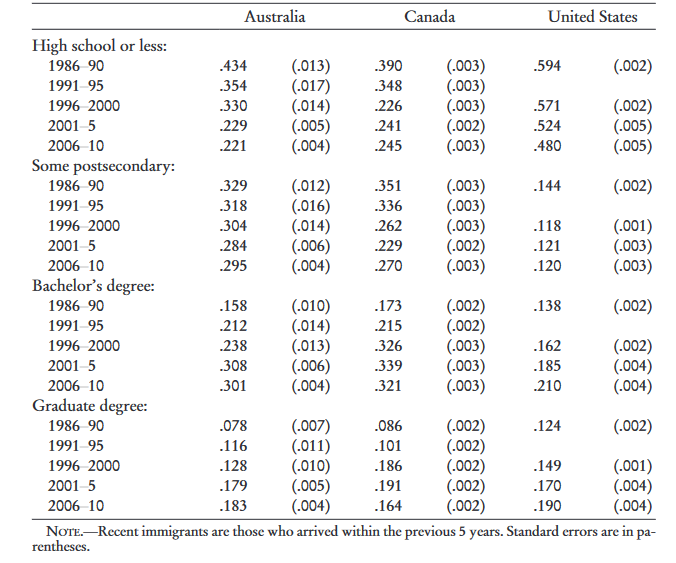
\includegraphics[width = \linewidth]{0828sugiyama/Table_1.png}
        \caption{ Education Distribution of Recent Immigrants by Education Group,Arrival Cohort, and Destination Country}
        \label{fig:my_label}
    \end{figure}
    
    The advantage focusing university-educated immigrants is that the mix of countries from which Australia, and Canadian, and US university-educated immigrants originate is more similar than it is less educated immigrants. This is evident in table 2.
    
    
    \begin{figure}
        \centering
        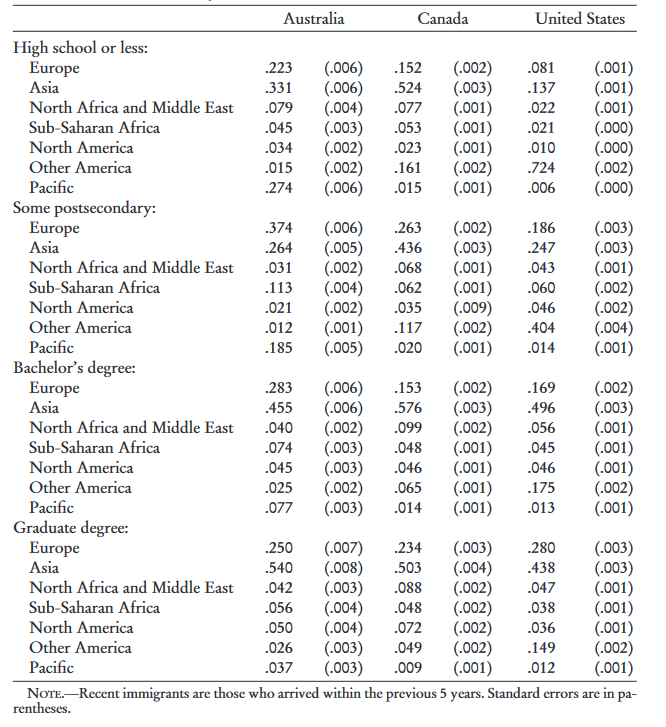
\includegraphics[width = \linewidth]{0828sugiyama/Table_2.png}
        \caption{Source Region Distribution of Recent Immigrants by Education Group and Destination Country}
        \label{fig:my_label}
    \end{figure}
    
    After imposing the full set of sample restriction, sample sizes of prime-age university-educated men is as follow: 20,030 (immigrant) and 37,112 (native-born) for Australia; 204,295 (immigrant) and 113,195 (native-born); and 144,315 (immigrant) and 113,195 (native-born) for United States.
    
    Table 3 represent sample mean of key feature.
    \begin{figure}
        \centering
        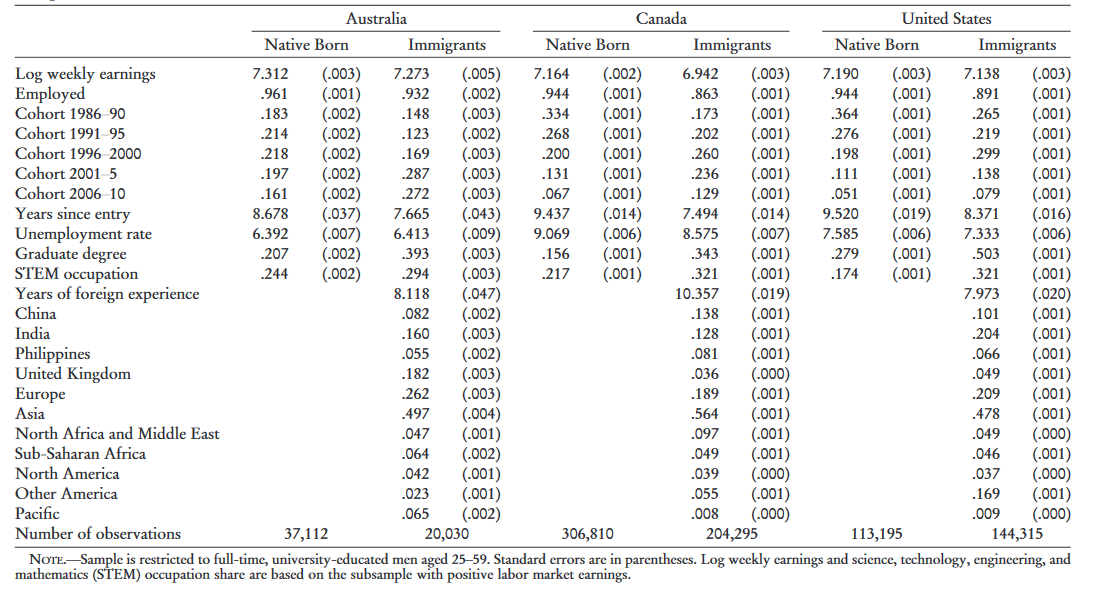
\includegraphics[width = \linewidth]{0828sugiyama/Table_3.png}
        \caption{Sample Means}
        \label{fig:my_label}
    \end{figure}
    
    
    {\bf Empirical Specification}
    
    A key challenge to estimate the effect of immigrant screening policy  on immigrant labor market outcomes is to account for different in broader labor market condition both within and across destination countries. 
    
    In this paper, following Green and Worswick’s (2012) approach of comparing recent immigrants to native-born new labor market entrants, the authors examine changes over time in the employment rates and earnings of new immigrants by estimating the following empirical specification:
    
    \begin{align}
    \begin{split}
         y_{ijrt} = &\alpha + \sum^{5}_{j=2}\beta_j C_j + f(yse_{jrt}) + \sum^{5}_{j=2}\delta_j (C_j\cdot yse_{jrt}) +\lambda_1 ur_{rt} + \pi grd_{ijr} +  X' \gamma  \\
        &+M_{ijr} \left[\sum^{5}_{j=1}\beta^m_j C_j +  \sum^{5}_{j=1} \delta^m_j(C_j\cdot yse_{jrt}) +\theta_1 f \ exp_{jrt} +\theta_2( f \ exp_{jrt}\cot \ yse_{jrt} )+\pi^m grd_{ijr}  \right] \\
        &+ \epsilon_{ijrt},
    \end{split}
    \end{align}
    
    where $y_{ijrt}$ is employment dummy variable or log weekly real earnings of individual $i$ from labor market entry cohort $j$ resident in geography $r$ and observed year $t$; $C_j$ is five cohort dummy labor market entry; $f(yse_{jt})$ is a quadratic profile of year since labor market entry common to immigrants and natives; $ur_{rt}$ is a de-trended regional unemployment rate; $grad_{ijr}$ is a graduate degree dummy variable; $X_{r}$ is a vector of geographic dummies indicating the city, state, or province of residence; $M_{ijr}$ is an immigrant dummy variable; $fexp_{ijrt}$ is year of foreign labor-experience ; $\epsilon_{ijrt}$ is random error term. 
    
    
    Of primary interest is the comparison of the estimates of the immigrant cohort effect $\beta^m$ across destination countries, in terms of both their historical values and their evolution over time.
    
    Assume that the level of real weekly earnings is equal to the product of an individual's skill ($Q_{ij}$) and the price of the price of that skill $(P_{ijrt})$. Log real weekly earnings are then given by $y_{ijrt }= p_{ijrt} + q_{ij}$. If the mean skill of native does not vary across the native born entry cohorts, so that $E(q_{ik}|j=k, M_{ijrt}=0)=E(q_{il}|j=l, M_{ijrt}=0)$ for all $k\neq l$, then Labor Market Performance of University-Education Immigrants
    
    \begin{align}
        \begin{split}
            \beta_k = &E[p_{ijr,t+k}|j=k, yse_{jrt}=0, M_{ijr, t+k}=0] \\
            &- E[p_{ijr}|j=0, yse_{jrt}=0, M_{ijr}=0],
        \end{split}
    \end{align}
     so that the native entry cohort effect capture the change in average skill price across cohort relative to the base cohort 0.
     If we further assume that immigrants face the same average skill prices as native within any period $t=t^*$, that is, $E(q_{ik}|t=t^*, M_{ijrt}=1)=E(q_{il}|t=t^*, M_{ijrt}=0)$, then 
     
     \begin{align}
        \begin{split}
            \beta^m_k = &E[p_{ijr,t+k}|j=k, yse_{jrt}=0, M_{ijr, t+k}=1] \\
            &- E[p_{ijr}|j=0, yse_{jrt}=0, M_{ijr}=0],
        \end{split}
    \end{align}
     so that the immigrant cohort effect capture difference in average skill between natives and immigrants who entered the labor market in the same period.
     
     The authors expect immigrant screening policies to have their primary effect by influencing this average skill level of university-educated immigrants. 
      
     
     The assumption that immigrants receive the same labor market returns to their skills is undoubtedly a strong one. There is compelling evidence from Canada that immigrants face labor market discrimination in recruiting based on their names (Oreopoulos 2011). However, this paper  is primarily interested in how employment rates and earnings of immigrants from a particular origin country have evolved differently in Australia, Canada, and the United States. The authors find it difficult to think of reasons why differences in the extent of discrimination against immigrants could explain these differences.
     
     \section{Results}
     
     The authors began analysis by comparing employment rate and log weekly earnings in the full sample of full-time, university-educated male workers. The estimates of $\beta_j$ in equation (1) are estimates of the expected employment rate of native-born workers in their first 5 years following labor market entry relative to native who entered in the 1986-90 period. 
     
     
    \begin{figure}
        \centering
        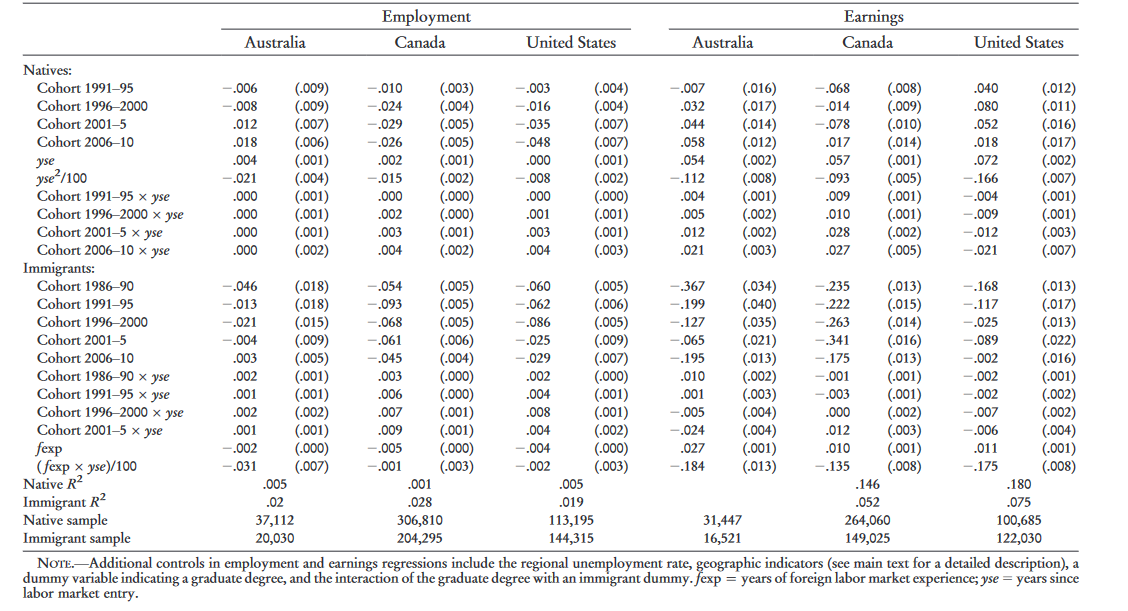
\includegraphics[width = \linewidth]{0828sugiyama/Table_4.png}
        \caption{Employment and Log Weekly Earnings Least-Squares Regressions}
        \label{fig:my_label}
    \end{figure}
    
    The estimates for earliest immigrant entry cohort (1986-1990) suggest little difference in the employment rate gap between the three countries. Australian gains, since the late 1990s, are more consist with the growing importance of two-step immigration.
    
    Similarly, for the United States, the gains in immigrant employment rates since the mid-1990s are consistent with the expansion of the H-1B.How-ever, they are also consistent with increasing US inequality and positive selectivity of US immigrants, particularly between 1996–2000 and 2001–5.
    
    
    In Canada, the policy reform have started since 1990s. This policy change lead to greater gains in employment rates with additional years since entry for Canadian immigrants.  
    
    Turning to earnings estimate, the results suggest earnings gaps for new university-educated immigrants in all three countries.
    
    The large improvement in Australian immigrant entry earnings between the 1986–90 and 1991–95cohorts (17 log points) therefore appears most consistent with increasing positive selectivity of Australian immigrants owing to rising skill returns.
    
    The US estimates point to a significant in-crease in the earnings of immigrants arriving in the 1996–2000 period and this is consist with expansion of H-1B program.
    
    
    The earnings performance of the most recent cohorts of Canadian  immigrants suggest a little gains for immigrants. This suggest Canada's its point system in the mid-2000s have been effective selective immigrants but there are still challenges for Canadian immigrants.  
    
     Comparing the estimated returns to years since entry in the earnings results in table 4 provides some evidence of this, but only for the 2001–5 cohort, whose entry earnings were exceptionally lo.
    
    The results from table 4 point to a substantial performance advantage for US university-educated immigrants in comparison to Australian and Canadian immigrants. 
    
    {\bf Quantile regression results}
    
    In figure 1, the authors examine whether these patterns are different at the lower and upper ends of the earnings. 
    
    \begin{figure}
        \centering
        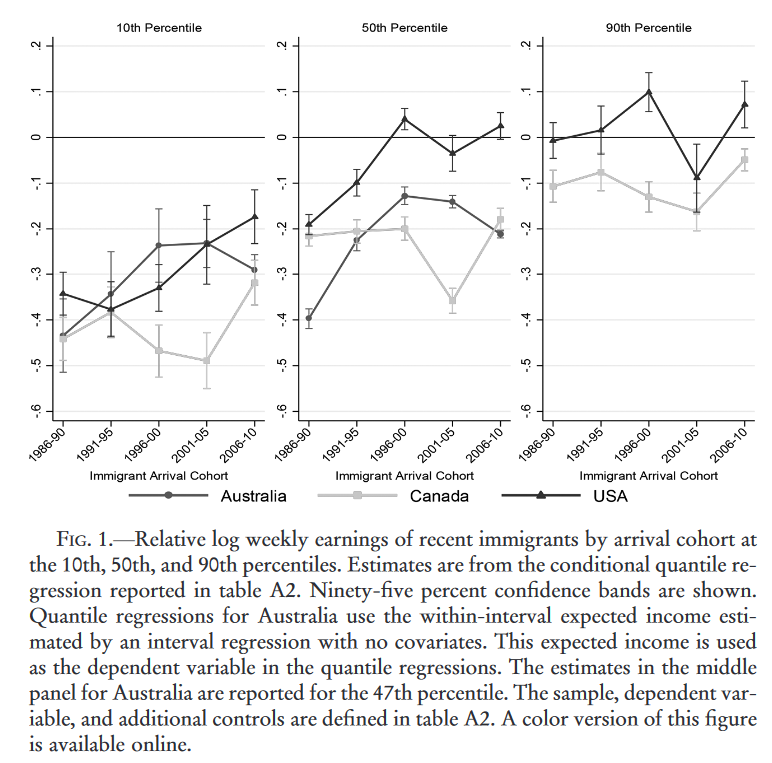
\includegraphics[width = \linewidth]{0828sugiyama/Figure_1.png}
        \caption{Relative log weekly earnings of recent immigrants by arrival cohort at the 10th, 50th, and 90th percentile}
        \label{fig:my_label}
    \end{figure}
    
    Figure 1 reveals two main results.
    \begin{itemize}
        \item The magnitude of the immigrant earnings gaps are mostly larger at the lower end of the distribution than at the top. For Canada, the gaps are particular large.
        \item To the extent that the improvements in immigrant entry earnings identified in table 4 reflect policy reforms, it appears that policy effects were not uniform over the immigrant earnings distribution.
    \end{itemize}
    In Australia,the gains are larger in the middle of the distribution, perhaps reflecting the growth of two-step immigration.
    
    In Canada, the improvement for the most recent arrival cohort is more evident at the lower end and middle of the distribution than at the top.
    
    The improvement in US immigrant earnings in the late 1990s appears strongest in the middle and top end of the distribution.
    
    {\bf The difference of source-countries}
    
    The current literature emphasize the importance of source-countries earnings distribution in understand difference in the performance of immigrant across destination countries.
    
    Figure 2 show relative immigrant entry estimates by country of origin.
    
    \begin{figure}
        \centering
        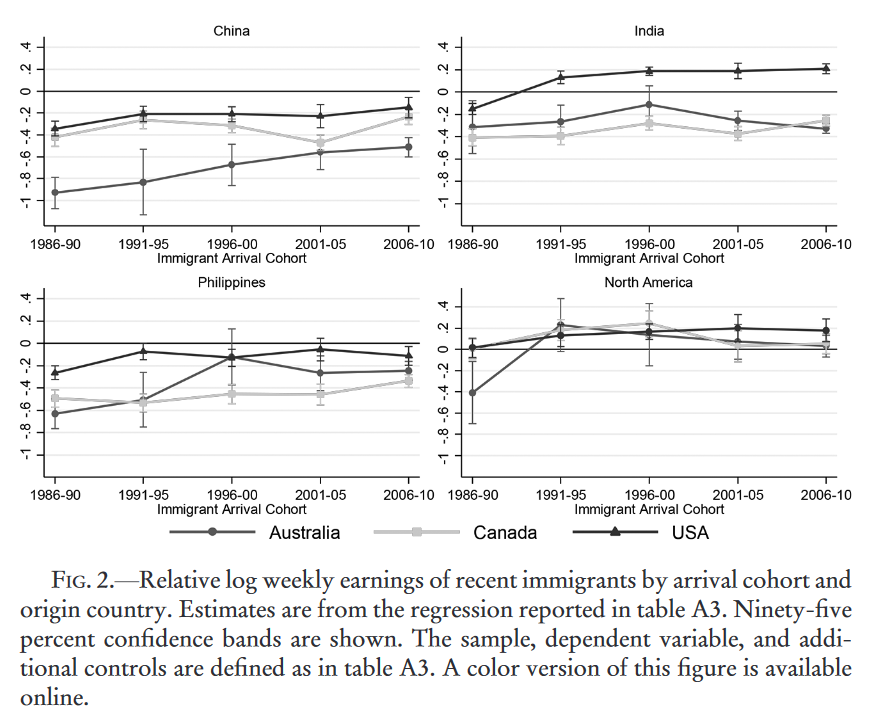
\includegraphics[width = \linewidth]{0828sugiyama/FIgure_2.png}
        \caption{Relative log weekly earnings of recent immigrants by arrival cohort and origin country. }
        \label{fig:my_label}
    \end{figure}
    The authors plot the results of three countries of origin with large enough samples : China, India,and the Philippines and add North America as an additional group, which includes US immigrants in Canada, Canadian immigrants in the United States, and Canadian and US immigrants in Australia. 
    
    Chinese university-educated immigrants fare substantially worse in Australia and much worse than the average Australian immigrants. However, their entry earnings have been improving for successive cohort consisting with increasing of selection policy. 
    
    
    Turning to Indian migrants, there is little evidence in the Australian or Canadian estimates of improving earnings performance consistent with selection policy reforms. In the United States, the entry earnings of recent Indians grew over the entire sample period.
    This results suggest the impact of H1-B program. These results seem likely to show the reason for the US advantage in table 4. In fact, it is possible that the H-1B program interacts in an important way with inequality.
    
    Similar to China, the level of inequality in the Philippines exceeded that in Australia, Canada, and the United States throughout the sample period.
    
    
    The estimates of immigrants born in Canada and the United States suggest earnings advantage relative to native-born new labor market entrances. These results once again emphasize the positive selectivity of skilled immigrants in the United States owing to higher returns to skill.
    
    {\bf Comparing immigrant STEM workers and non-STEM workers}
    
   The exceptional performance of Indian immigrants in the United States suggests that immigrant selection policies may have an important influence on the occupational background of immigrants. To examine this issue, the authors consider the entry earnings of workers in STEM and non-STEM occupation separately. The results of this analysis are presented in figure 3.
   
   \begin{figure}
        \centering
        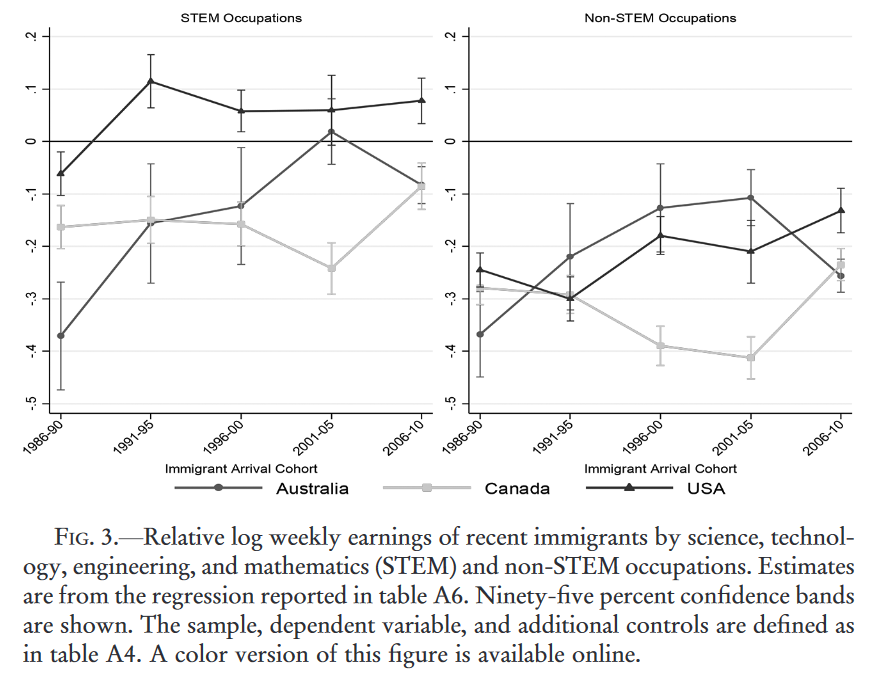
\includegraphics[width = \linewidth]{0828sugiyama/FIgure_3.png}
        \caption{Relative log weekly earnings of recent immigrants by science, technology, engineering, and mathematics (STEM) and non-STEM occupations. }
        \label{fig:my_label}
    \end{figure}
    
    \begin{itemize}
        \item Immigrant STEM workers in three countries tend to outperform their non-STEM workers
        \item The earnings gains of Australian immigrants in the late 1990s and early 2000 are evident among STEM and non-STEM workers.   
        \item There is less clear evidence of improvement among US STEM and non-STEM workers than in the full sample of all US immigrants in table 4.This implies that an important part of the overall US gains reflects a compositional shift in skilled immigration toward STEM workers. 
    \end{itemize}
    
    
    \section{Conclusion}
    This paper show two main finding as follow:
    
    \begin{enumerate}
        \item In contrast to much of the current literature, the authors find evidence of the improving relative and absolute labor market earnings of university-educated immigrant men through the 1990s and 2000s in Australia, Canada, and the United States. 
        \item Estimates point to a large and persistent performance advantage in the full-time earnings of university-educated only US. This advantage is represented by the estimates of Indian immigrants and immigrant STEM workers.
    \end{enumerate}
      
    One interpretation of the exceptional performance of US skilled immigrants is that two-step immigration lead to superior labor market outcomes. However, there are three reasons that the authors think this interpretation is lacking.
    
    \begin{itemize}
        \item US advantage is evident only in full-time earnings.
        \item Comparing postimmigeration earnings growth is not short-term phenomenon.
        \item Similarly, however, the two-step policy is improved in  Australia, but the Australian immigrants earning gains less than American ones.
    \end{itemize}
    
    It also seems unlikely that the large US performance advantage reflects lower levels of labor market discrimination in the United States (Duleep and Regets 1992).
    
    \biblio
    
\end{document}